\begin{figure}
    \begin{center}
    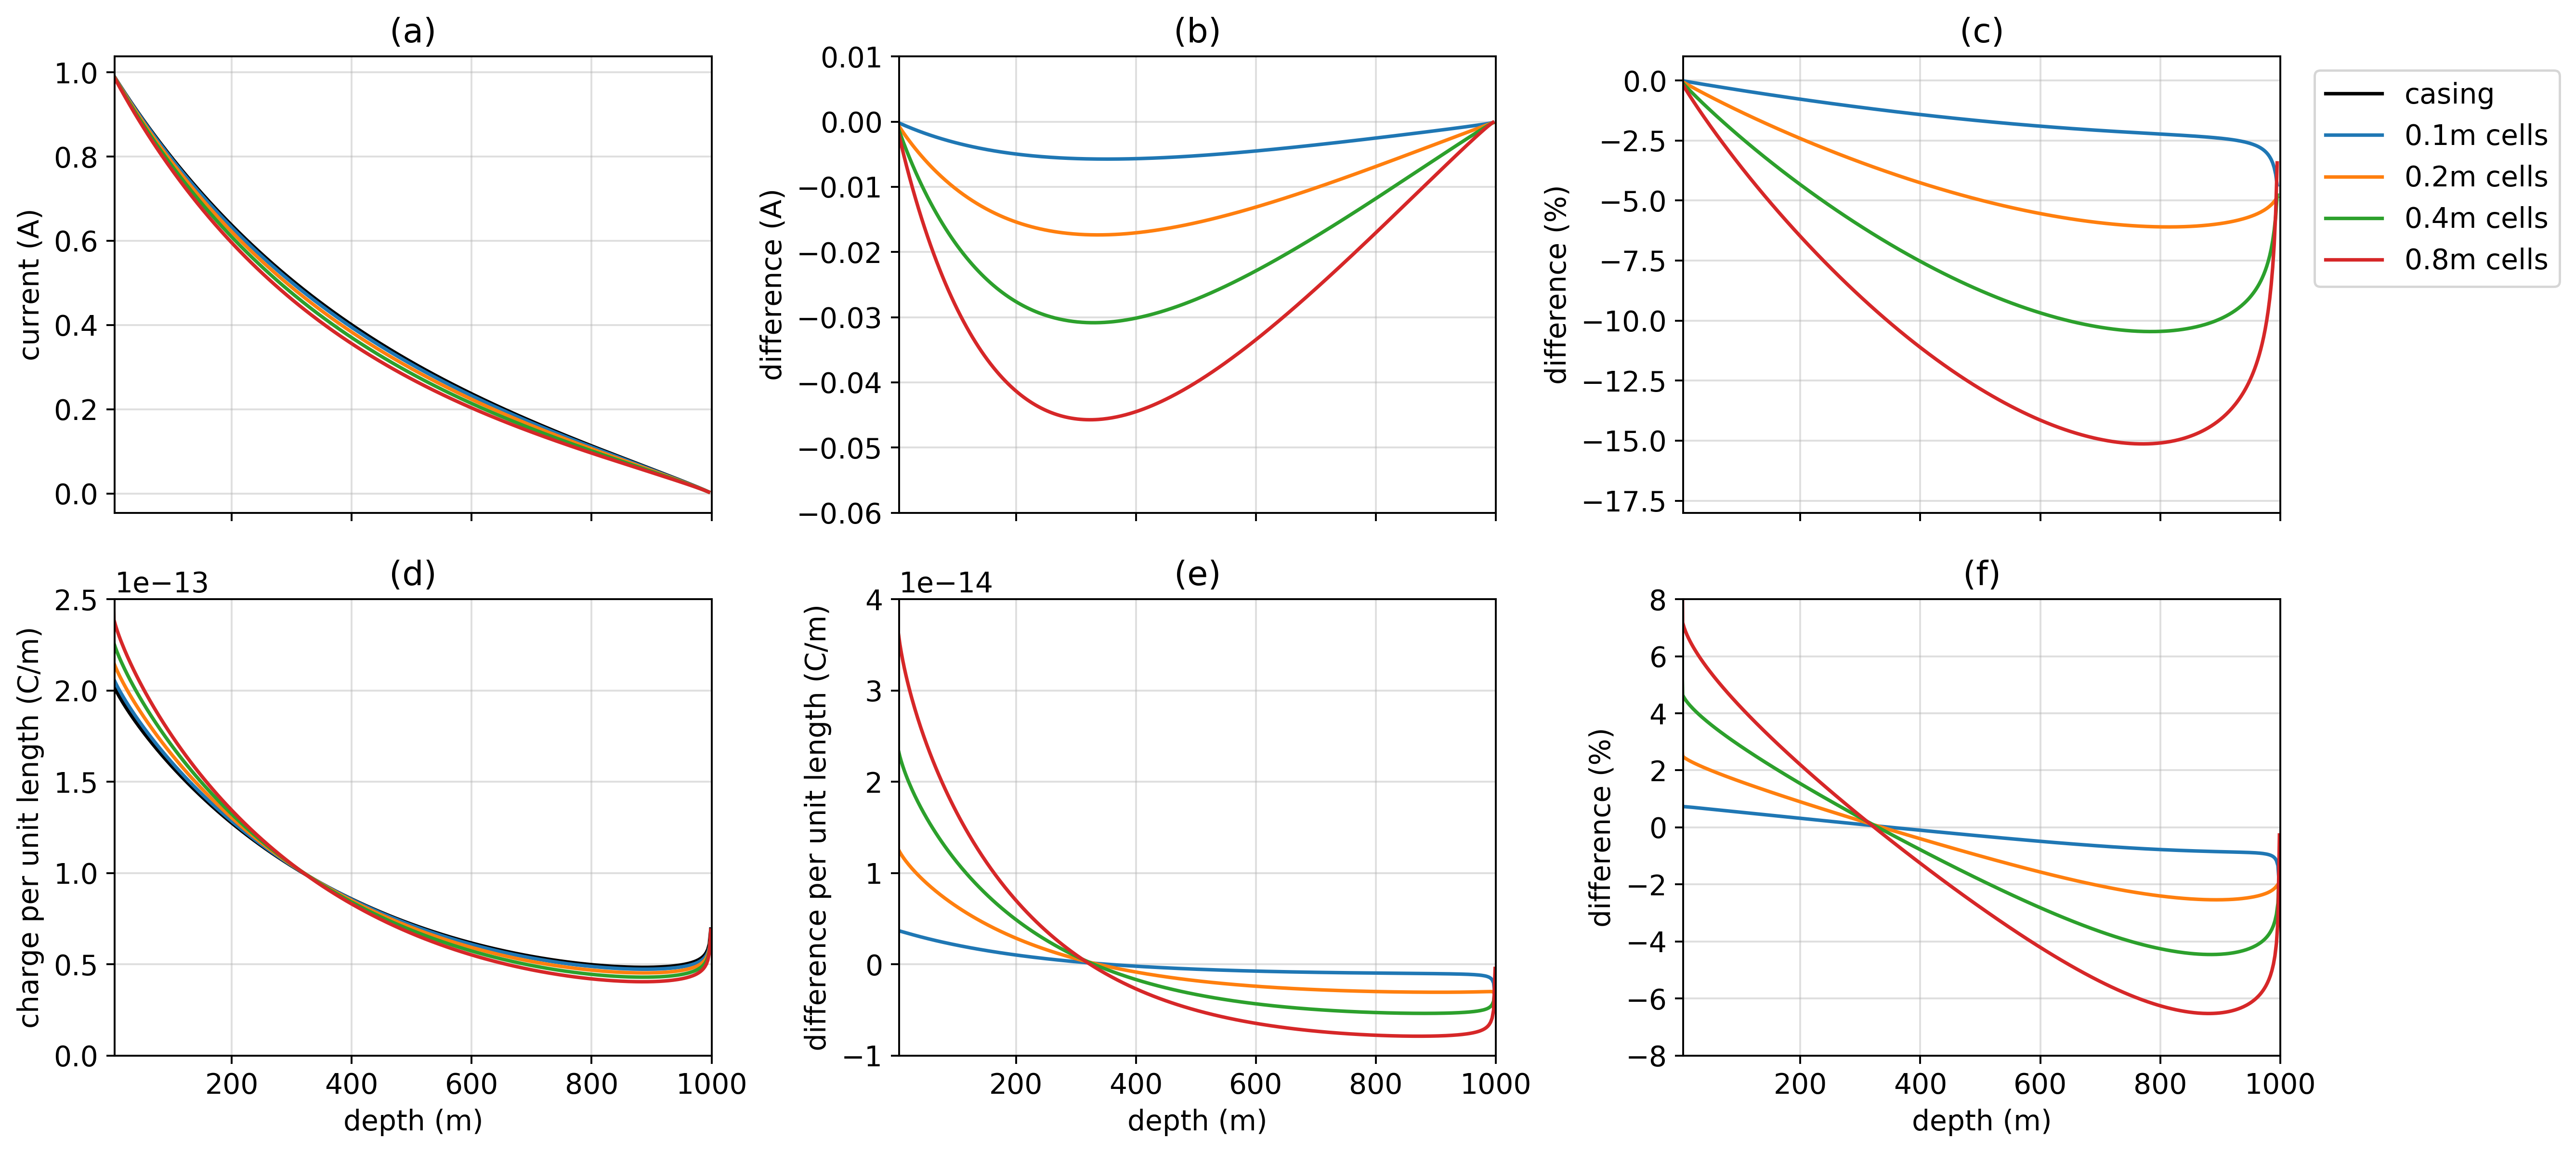
\includegraphics[width=\textwidth]{figures/approximating_wells_cartesian.png}
    \end{center}
\caption{
    Currents (top row) and charges (bottom row) along the length of
    a steel cased well. The ``true'' hollow-cased well is simulated on a
    3D cylindrical mesh and has 4 cells across the width of the casing thickness (black line).
    The colored lines correspond to the currents and charges computed along the
    well represented on a cartesian mesh with cell widths shown in the legend.
    The finest vertical discretization is 2.5 m in all simulations. To represent the
    hollow cased well on the cartesian mesh, the cells intersected by the casing are assigned
    a conductivity that preserves the product of the conductivity and cross-sectional area of the well.
    In (a), we show the vertical current in the casing,
    (b) shows the difference from the true, hollow-cased well
    in the vertical current within the casing, and (c) shows that difference as a percentage
    of the true currents. In (d), we show the charge per unit length along the casing, (e)
    shows the difference from the true, hollow-cased well and (e) shows that differences as
    a percentage of the true charge distribution.
}
\label{fig:approximating_wells_cartesian}
\end{figure}
